\chapter{System Overview}
\label{ch:System Overview}
The system modeled is a web-enabled password manager that resides on a
tamper resistant USB thumb drive, modeled after the
IronKey\texttrademark~secure USB thumb drive. The password manager
allows for a user to enjoy the benefits of a secure offline password
manager with the option of receiving software and firmware updates from the
cloud. The USB device also hosts an embedded crypto system which can be
leveraged to provide powerful cryptographic tools which provide some assurance
that the tools have not been compromised. Because security is the primary objective, the password file (the file which stores user names, passwords, and their associated applications, appliances, or domains) is not written to persistent media outside the USB device.

\begin{marginfigure}%
\centering
  
\includegraphics[width=0.25\linewidth]{s1000-vertical}
  \caption{Picture of the IronKey USB drive.  More information can be
found at \url{www.ironkey.com}}
  \label{fig:ik}
\end{marginfigure}



\section{System Description}
\label{sec:sysdesc}

The concept of operation is for the user to, after having inserted the device into a computer, launch the provided trusted application from the USB device, which has been mounted as a CD-ROM.  The application's public key is sent to the computer along with the application executable, and used to establish a temporary encrypted session with the USB (in which the corresponding private key is stored).  Within the temporary session, a random shared key is generated by the USB device and passed to the application to establish the secure application session.  Once the application is running, the user is in a secure but anonymous session with the USB device.  From this point, the user can choose to (a) submit a master password to the application in order to access his/her password store, (b) perform a secure software update on the device, or (c) perform a hard reset of the device, restoring the device to factory condition and losing any password store data.
\begin{enumerate}
    \item When the user submits his/her master password, the USB device will attempt to decrypt a header file stored on the device.  If successful, the device will initiate a secure user session with the application, encrypted using a the symmetric secure application key as well as a key derived from the user's password.  In this session, the user (via the application) may perform privileged operations with the password store file.
    \item When the user performs a secure software update, the application interrogates the web server as to the latest software release and downloads the digitally signed file.  Next, the application sends the file to the USB device for the update.  Within the USB device, the updated software is checked using the factory's public key and, if authentic, generates a new public/private key pair to store on the device, overwriting the current version of the software.  Finally, the USB device forces a restart of the device and the application using the new version.
    \item When the user elects to perform a hard reset on the device, the device overwrites the header file and password store file with a stored from-factory version, thereby permanently erasing any previously stored user password information and restoring the device to a factory state.
\end{enumerate}
\par The USB device firmware and software can be updated via a secure Internet
channel which accesses a webserver to download the device files to the USB
device.  Following download, the device authenticates the downloaded files and
updates the device.
The way to save the password via the password manager is straightforward. The
password is passed along with the corresponding key (e.g. a website, a username,
hostname, \dots) to the password manager when the secure user session is
setup as shown in Figures~\ref{fig:dfd_app} and ~\ref{fig:dfd_usb}. The key
must be unique. Once
the password is stored with the corresponding key to the encrypted partition in
the USB, a user can retrieve the password with the unique given key during the
secure user session. The retrieved password can be blinded out and copied to the
temporary memory of the system (e.g. clipboard) for users' convenience. Of
course, if a user inquires, the password can be displayed in a plain text but
preferably in an image format.

\begin{figure}
    \centering
    \includegraphics{DFD_Main}
    \caption{Main System Data Flow Diagram}
    \label{fig:dfd_main}
\end{figure}
\begin{figure*}
    \centering
    \includegraphics[width=\linewidth]{DFD_App}
    \caption{System Data Flow Diagram in the App side}
    \label{fig:dfd_app}
\end{figure*}

\begin{figure*}
    \centering
    \includegraphics[width=\linewidth]{DFD_USB}
    \caption{System Data Flow Diagram in the USB side}
    \label{fig:dfd_usb}
\end{figure*}

%\begin{figure*}
%    \centering
%    \includegraphics[width=0.8\linewidth]{webservdfd1}
%    \caption{System Data Flow Diagram for the Webserver}
%    \label{fig:wsdfd1}
%\end{figure*}


\begin{figure*}
    \centering
    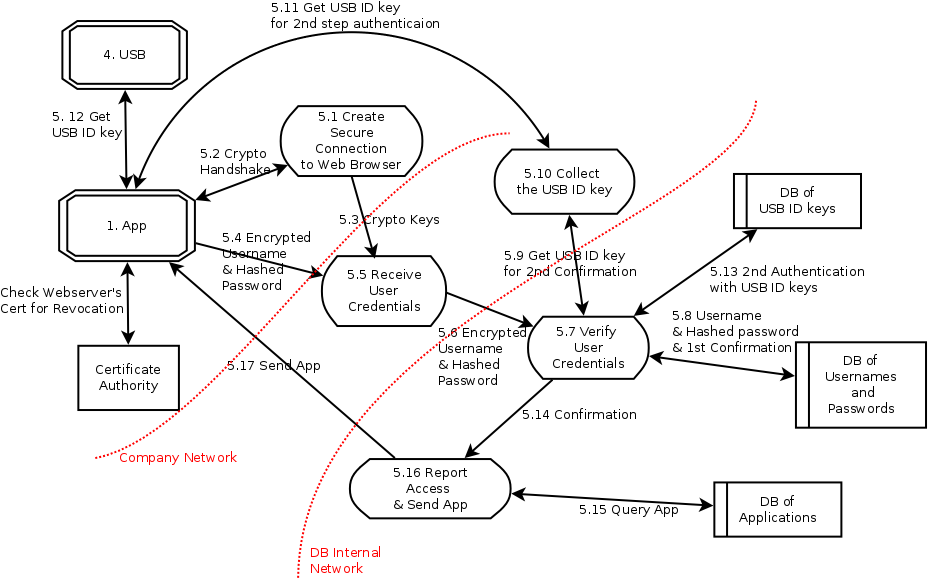
\includegraphics[width=0.8\linewidth]{DFD_Webserver}
    \caption{System Data Flow Diagram for the Webserverer}
    \label{fig:wsdfd}
\end{figure*}

The Password manager consists of two major components, the USB device and a User
Application. The USB device when plugged in the system is loaded as a CD
ROM. The Get/Load function from the application gets the public key and begins
the message
encryption. Once the user application is authenticated and loaded there can be 4
possibilities:
\begin{enumerate}
\item The password manager is used for the first time by the user
\item Correct credentials are entered by the user
\item Incorrect credentials are entered by the user
\item User enters incorrect credentials multiple times
\end{enumerate}

When the user uses the iron key for the first time, the header is decrypted with
the default key. Once the header decrypt is successful the user is forced to
reset the default password. When correct credentials are entered by the user,
the password key is sent to the USB which then decrypts the header with that
key.  Once the header is decrypted a a user session is started. The counter
which stores the number of invalid attempts is reset.The user has the option to
update the user password. The decrypted file is read into the memory and a new
password key and password file/header is written to the USB.A pair of key and
password is stored in the USB device. The password is queried from the USB
device using the given key.

If the user enters an invalid credentials, the header decrypt fails and the
password try counter is incremented.\marginnote{The USB itself does not possess
any logging capability save for the try counter which also serves as an
initiator to clear the system after a number of incorrect tries.} The user is
then prompted to enter a correct password. When a user enters a wrong password
multiple times which is equal to some threshold value, the reset counter
overwrites the header and password file by default.

The user application can be updated. When the update is successful, the USB is
updated and a force restart happens with the new version.When an update fails
the current version of the app is maintained.

The system data flow diagram is shown in figure \ref{fig:dfd_main}.


\section{Functional Requirements}
\label{sec:funcreq}
The functional requirements of the system are as follows:
\begin{enumerate}
    \item{Physically protect the USB against known tamper attacks including
physical attacks and USB electrical channel attacks.}\sidenote{We do not
enumerate all the possible USB physical and electrical attacks, nor do we
describe in detail the mitigations to these attacks.  It is assumed that
appropriate hardware antitamper features are incorporated into the USB design.}
    \item{Host all cryptography on the USB device.}
    \item{Allow for remote updates of USB software and firmware.}
    \item{Initiate device wipe after a set number of incorrect login attempts.}
    \item{Allow for the secure storage and retrieval of user websites and login
information.}
    \item{Provide for a secure, random password generator capability.}
\end{enumerate}
